\documentclass[12pt]{article}
\usepackage[spanish]{babel}
\usepackage{natbib}
\usepackage{pdflscape}
\usepackage{url}
\usepackage{float}
\usepackage[utf8]{inputenc}
\usepackage{amsmath}
\usepackage{graphicx}
\usepackage{fancyhdr}
\usepackage{longtable}
\usepackage{vmargin}
\usepackage{listings}
\usepackage{hyperref}
\usepackage{multirow}
\setmarginsrb{2 cm}{2.5 cm}{2 cm}{2.5 cm}{1 cm}{1.5 cm}{1 cm}{1.5 cm}

\title{Tarea - 03}
\date{\today}

\makeatletter
\let\thetitle\@title
\let\theauthor\@author
\let\thedate\@date
\makeatother

\pagestyle{fancy}
\fancyhf{}
\rhead{\theauthor}
\lhead{\thetitle}
\cfoot{\thepage}

\addto\captionsspanish{
  \renewcommand{\contentsname}%
    {Tabla de contenido}%
}

\begin{document}
    \pagestyle{fancy}
    \fancyhf{}

    \lhead{\begin{picture}(0,0) \put(0,0){
\includegraphics[width=30mm]{images/Logo2.png}} \end{picture}}
    \renewcommand{\headrulewidth}{0.7pt}
    \fancyhead[R]{Procesamiento de lenguaje natural - Tarea 02}
\fancyfoot[R]{\thepage}

\begin{titlepage}
	\centering
    
\includegraphics[scale = 0.45]{images/Logo.png}\\[0.5 cm]	% University Logo
    \textsc{\large Universidad de los Andes\\
        \vspace{0.2cm} 
        Facultad de ingeniería\\
        \vspace{0.3cm} 
        Tarea 03}\\[2.0 cm]	% University Name
	\textsc{\Large Procesamiento de lenguaje natural}\\[0.5 cm]
	% Course Code
	\rule{\linewidth}{0.2 mm} \\[0.4 cm]
	{ \LARGE \bfseries \thetitle}\\
	\rule{\linewidth}{0.2 mm} \\[1.5 cm]
	
	\large
			\emph{Presentado por:} \\
			Juan David García Hernández\\
			Nicolás Rocha Pacheco\\
			César Daniel Garrido Urbano\\
	\vfill
	\large
			\emph{Presentado a:}\\
			Rubén Francisco Manrique Piramanrique\\
\end{titlepage}

\thispagestyle{empty}
\tableofcontents
\pagebreak

\setcounter{page}{1}

\section{Introducción}
\section{Preprocesamiento}

Antes de iniciar con el proceso de construcción de \textit{embeddings} y modelos de clasificación se realizó una estandarización o preprocesamiento a los datos de ambos \textit{datasets}. Este se puede encontrar en el cuaderno adjunto  \texttt{preprocessing.iynb}. Se empezó por importar los diálogos de ambas series, los cuales se encontraban en formatos distintos. \\

Por un lado, para el \textit{dataset} de Los Simpsons, los datos ya se encontraban discriminados por personaje, por lo que el único trabajo que se hizo fue el de seleccionar los dialogos de los 4 personajes principales (Homero, Marge, Bart y Lisa Simpson). Por otro lado, para el \textit{dataset} de Friends, se tenían el script crudo de cada uno de los episodios. De esta manera se leyeron todos los archivos verificando su contenido en cada línea. En caso de encontrar alguno de los personajes principales (Rachel, Ross, Chandler, Monica, Joey o Phoebe) se agregaba el contenido seguido de los dos puntos \textit{(:)} y se le agregaba la etiqueta del personaje. \\

Así las cosas, se obtuvieron el siguiente número de sentencias (o frases) por cada uno de los personajes principales (véase cuadro \ref{tab:dist-datos}). En estas se observa que la distribución de las clases es similar para tres de los cuatro personajes de los Simpsons. No obstante, Homero acapara poco más del 40\% de las sentencias, lo que sugiere un desbalance considerable en el caso de este \textit{dataset}. Por el lado de la serie de Friends, se observa una distribución mucho más balanceada de las clases, con una diferencia menor al $4\%$ entre la clase con más datos y la de menos datos. \\

\begin{table}[H]
\caption{Distribución de las clases (número de sentencias para cada personaje) en cada uno de los \textit{datasets}.}
\label{tab:dist-datos}
\centering
\begin{minipage}{0.45\textwidth}
\centering
\begin{tabular}{|l|l|}
\hline
\textbf{Character} & \textbf{N° Sentences} \\ \hline
Homer & 27850 \\ \hline
Marge & 13172 \\ \hline
Bart & 12995 \\ \hline
Lisa & 10756 \\ \hline
\end{tabular}
\caption*{a) Simpsons }

\end{minipage}\hfill
\begin{minipage}{0.45\textwidth}
\centering
\begin{tabular}{|l|l|}
\hline
\textbf{Character} & \textbf{N° Sentences} \\ \hline
Rachel & 8506 \\ \hline
Ross & 8262 \\ \hline
Chandler & 7686 \\ \hline
Moncia & 7620 \\ \hline
Joey & 7572 \\ \hline
Phoebe & 6831 \\ \hline
\end{tabular}
\caption*{b) Friends}

\end{minipage}

\end{table}

Ahora bien, a cada una de las sentencias se les aplico una estandarización la cual consistió en los siguientes procesos:

\begin{itemize}
    \item \textbf{lower case:} Las letras de todos los términos se transformaron a minúsculas.
    
    \item \textbf{colloquial term removal:} Se expandieron contracciones coloquiales (ejemplo: la expreisón \textit{don't} se reemplazo por \textit{do not}).
    
    \item \textbf{tokenización:} Se tokenizaron las palabras con el tokenizador \texttt{RegexpTokenizer} de \texttt{nltk}, el cual elimina todo signo de puntuación.
        
    \item \textbf{simple lematization:} Se redujo cada uno de los términos a su raíz con el lematizador \texttt{WordNetLematizer} de \texttt{nltk}.
    
\end{itemize}

Dado que para este trabajo las palabras se modelaran con \textit{embeddings} y no con un modelo de palabras de \textit{Bag of Words} (BOW) el preprocesamiento fue realmente simple y no se decidió remover stop words. Una vez realizada esta estandarización se obtuvo el tamaño de las frases (número de tokens en cada sentencia) para cada uno de los \textit{datasets}. Esto con el fin de tener una idea de cuantos términos (o \textit{tokens}) había en cada frase (véase figura \ref{fig:simpsons_hist} - \ref{fig:friends_hist}), algo de especial importancia al momento de realizar el \textit{padding} de las sentencias.  \\

\begin{figure}[H]
    \centering
    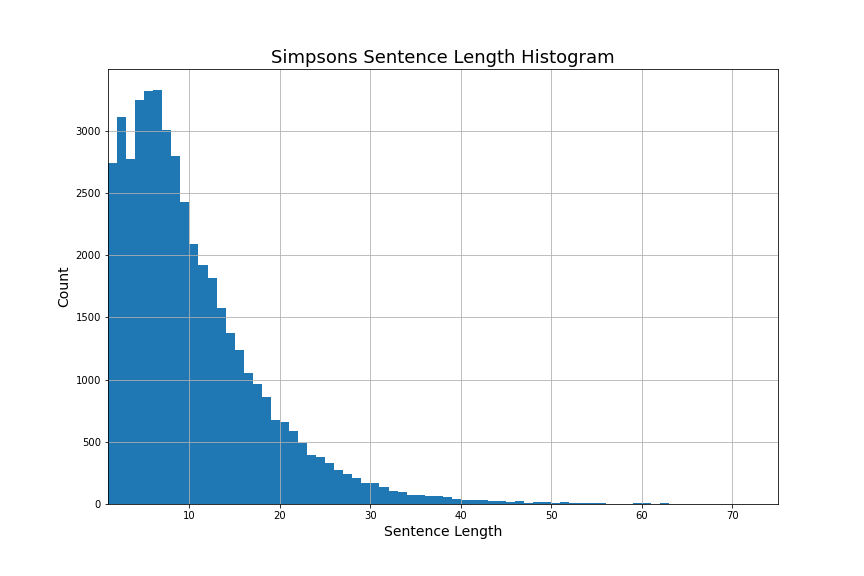
\includegraphics[width=0.95\textwidth]{results/preprocessing/simpsons_hist.png}
    \caption{Tamaño de las frases en los diálogos de los Simpsons (promedio = $9.93$, media = $8$).}
    \label{fig:simpsons_hist}
\end{figure}

Adicionalmente, en este punto también se separaron de una vez los \textit{datasets} en \textit{sets} de entrenamiento (\textit{train}), validación (\textit{val}) y prueba (\textit{test}), con una distribución de 70\%, 15\% y 15\% respectivamente. Esto con el fin de entrenar los modelos con un grupo de datos, definir su arquitectura y ajustar sus parámetros con otro grupo de datos y realizar la prueba definitiva de su desempeño con un último grupo de datos. 


\begin{figure}[H]
    \centering
    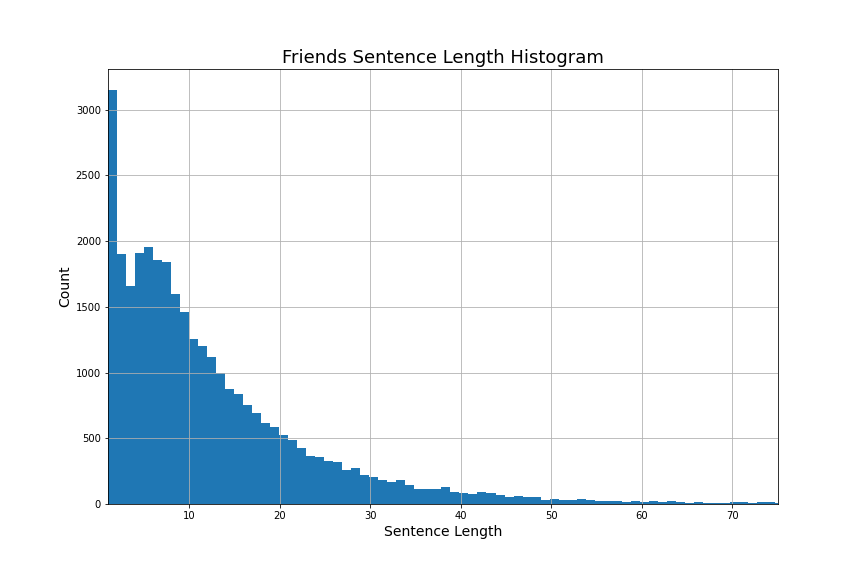
\includegraphics[width=0.95\textwidth]{results/preprocessing/friends_hist.png}
    \caption{Tamaño de las frases en los diálogos de la serie \textit{Friends} (promedio = $12.52$, media = $9$).}
    \label{fig:friends_hist}
\end{figure}

\newpage
\section{\textit{Embeddings}}

gesnim word2vec model

Parameters:
\begin{itemize}
    \item Embedding Size:
    
    \item Window:
    
    \item Min Count:
    
    \item SG:
    
    \item Negative:
\end{itemize}

\subsection{2D Plots}

PCA

\subsubsection{Simpsons Dataset}



\begin{figure}[H]
\centering
\begin{minipage}{0.45\textwidth}
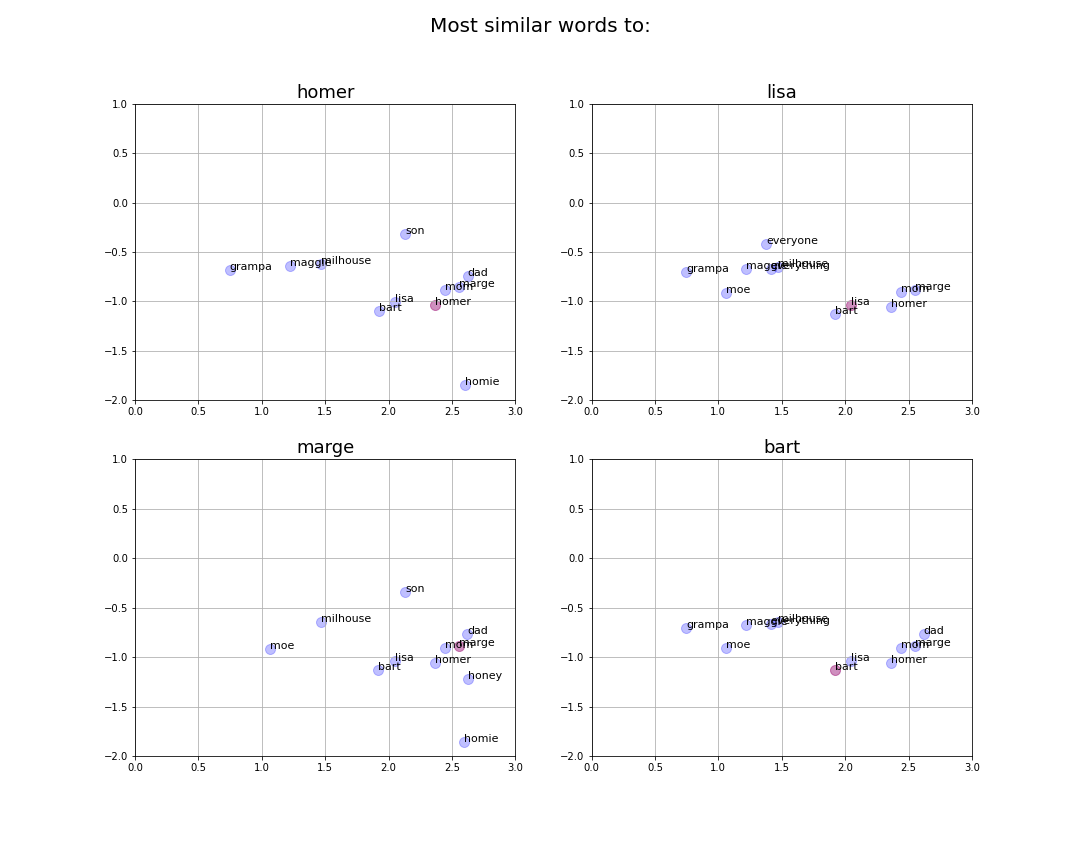
\includegraphics[trim=4.2cm 3cm 3.7cm 3cm, clip=true, width=\textwidth]{results/embeddings/simpsons_similar_15.png}
\caption*{a) DIM = 15}
\end{minipage}\hfill
\begin{minipage}{0.45\textwidth}
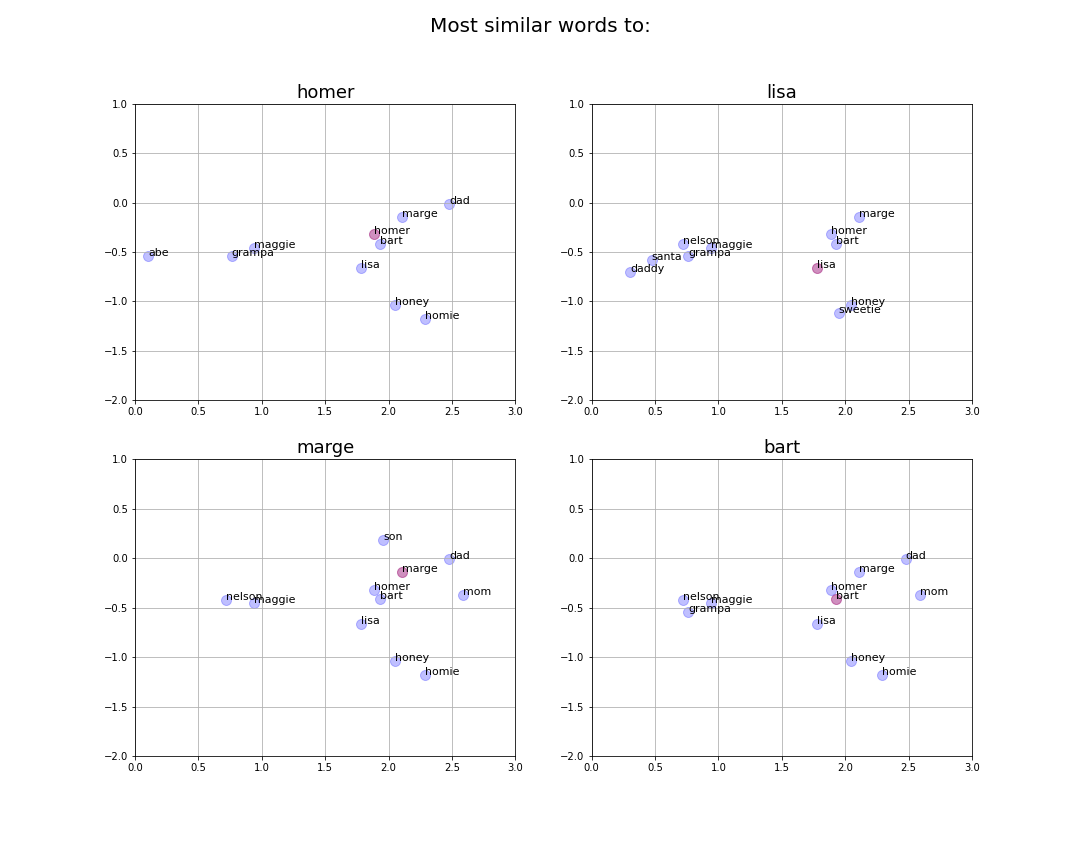
\includegraphics[trim=4.2cm 3cm 3.7cm 3cm, clip=true, width=\textwidth]{results/embeddings/simpsons_similar_75.png}
\caption*{b) DIM = 75}
\end{minipage}\par
\vskip\floatsep% normal separation between figures
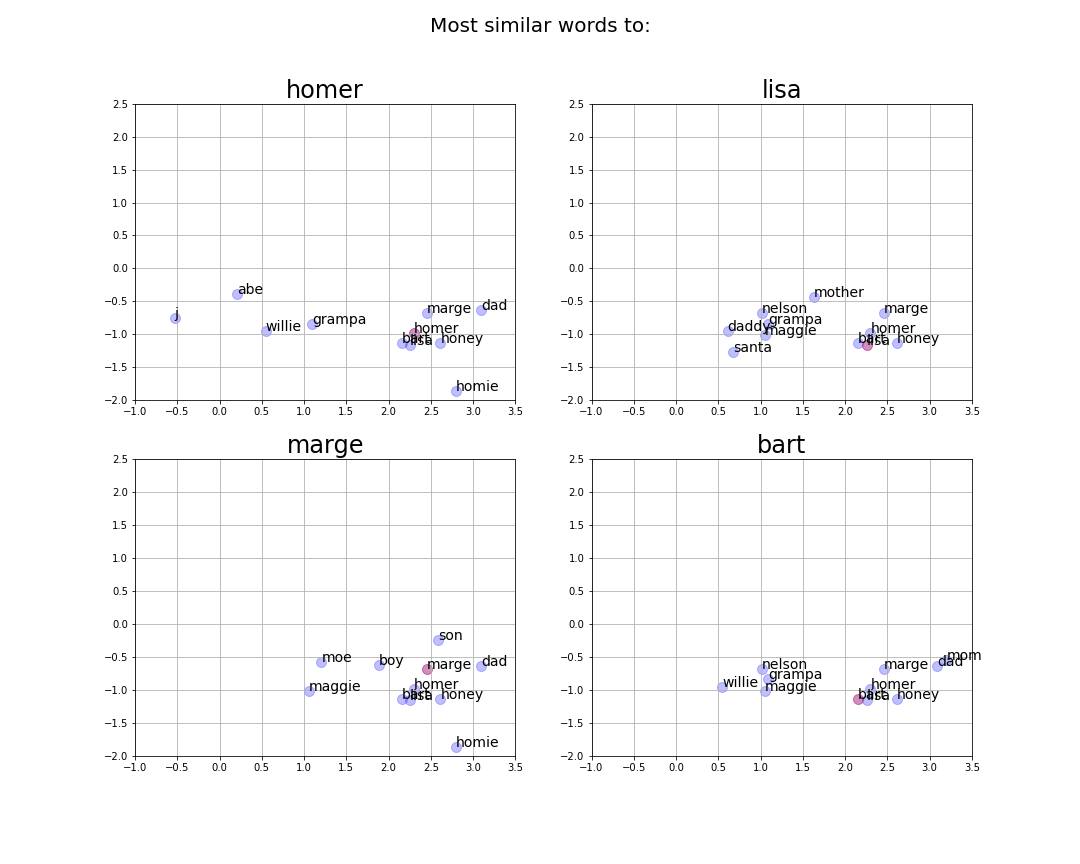
\includegraphics[trim=4.2cm 3cm 3.7cm 3cm, clip=true, width=0.45\textwidth]{results/embeddings/simpsons_similar_150.png}
\caption*{c) DIM = 150}
\caption{\textit{Embeddings} de los personajes principales de los Simpsons y los términos más similares proyectados en un plano 2D para distintos tamaño de embedding}
\label{fig:simpsons_sim_words}

\end{figure}


\subsubsection{Friends Dataset}

\begin{figure}[H]

\centering
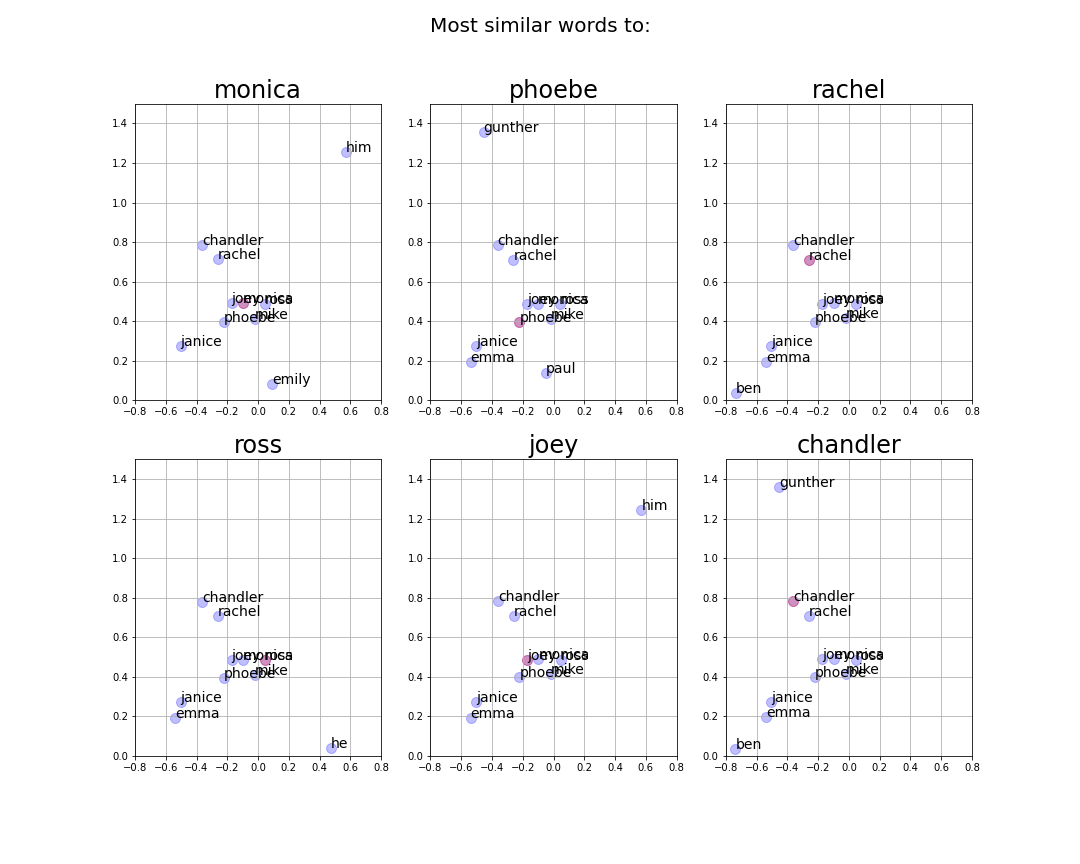
\includegraphics[trim=3cm 0cm 3cm 0cm, clip=true, width=.32\textwidth]{results/embeddings/friends_similar_15.png}\hfill
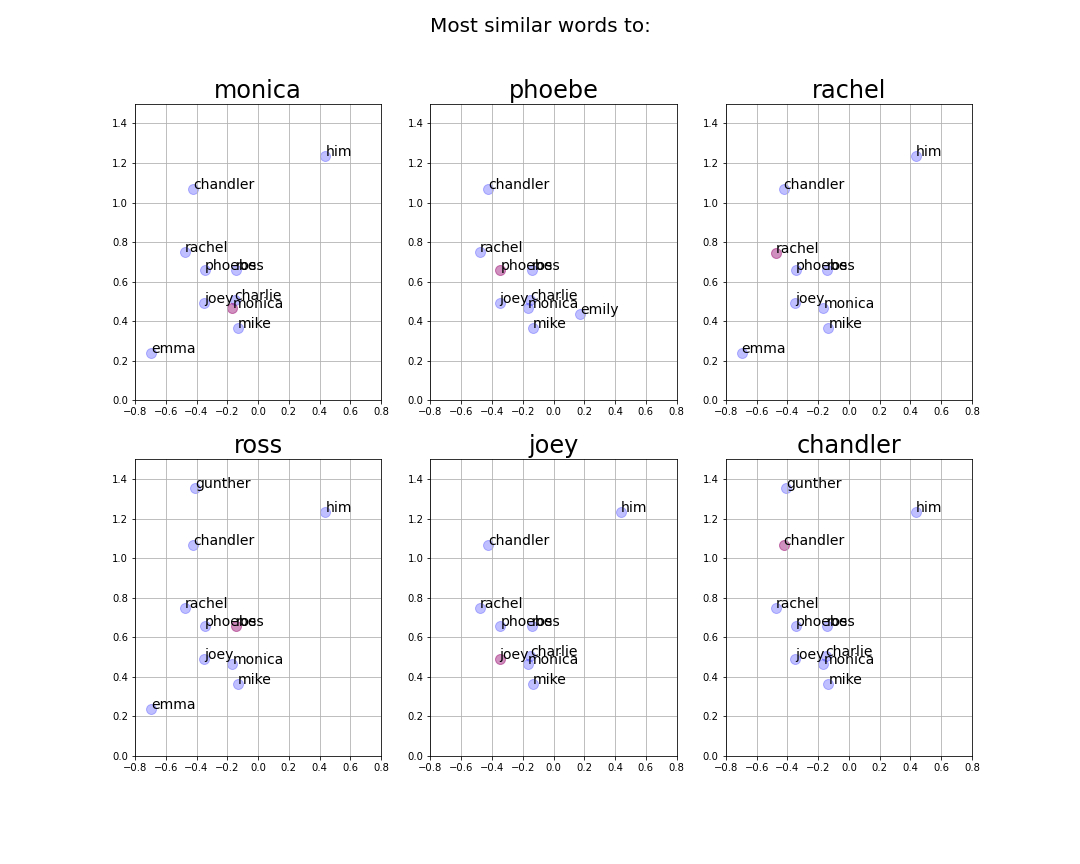
\includegraphics[trim=4cm 0cm 3.5cm 0cm, clip=true, width=.3\textwidth]{results/embeddings/friends_similar_75.png}\hfill
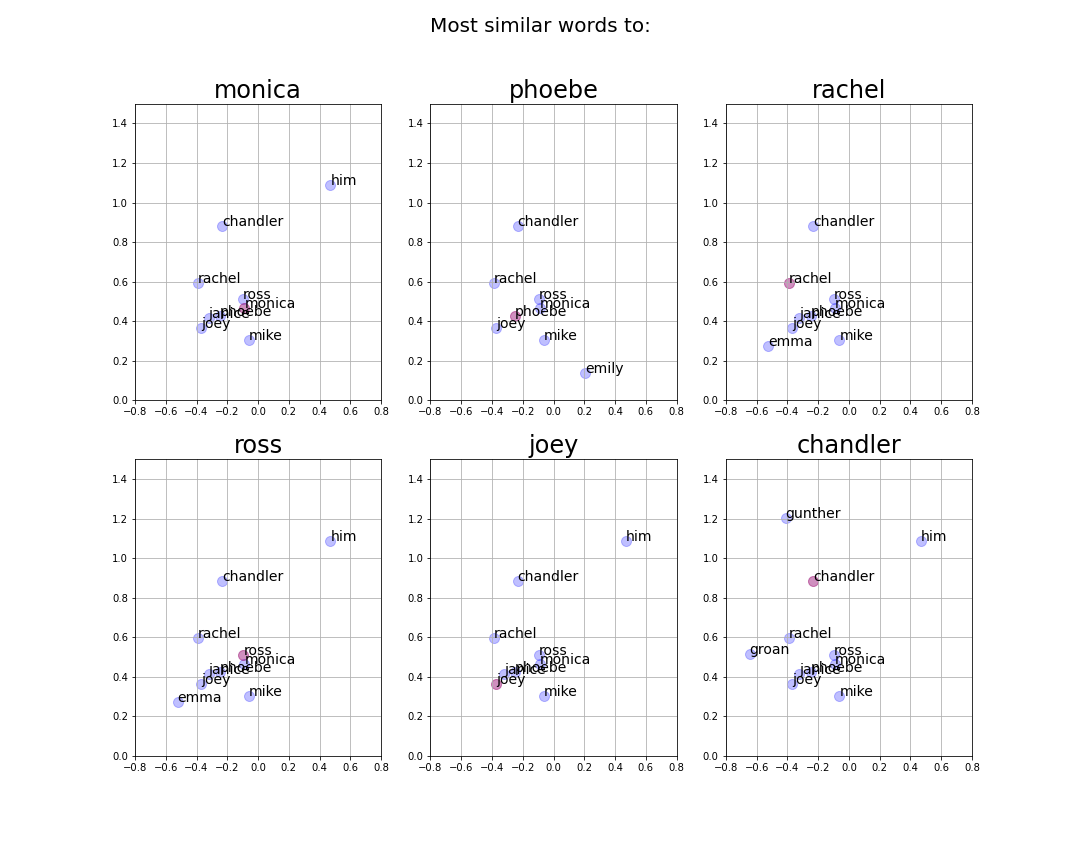
\includegraphics[trim=3cm 0cm 3cm 0cm, clip=true, width=.3\textwidth]{results/embeddings/friends_similar_150.png}
\caption{Embeddings de los personajes principales de Friends y los términos más similares, proyectados a un plano 2D }
\label{fig:friends_sim_words}

\end{figure}

\subsection{Interesting Relations}
\begin{itemize}
    \item Similaridad
    
    \item Analogía 
    
    \item Coincidencia (\textit{doesn't match})
\end{itemize}

\subsubsection{Simpsons Dataset}

\begin{figure}[H]
    \centering
    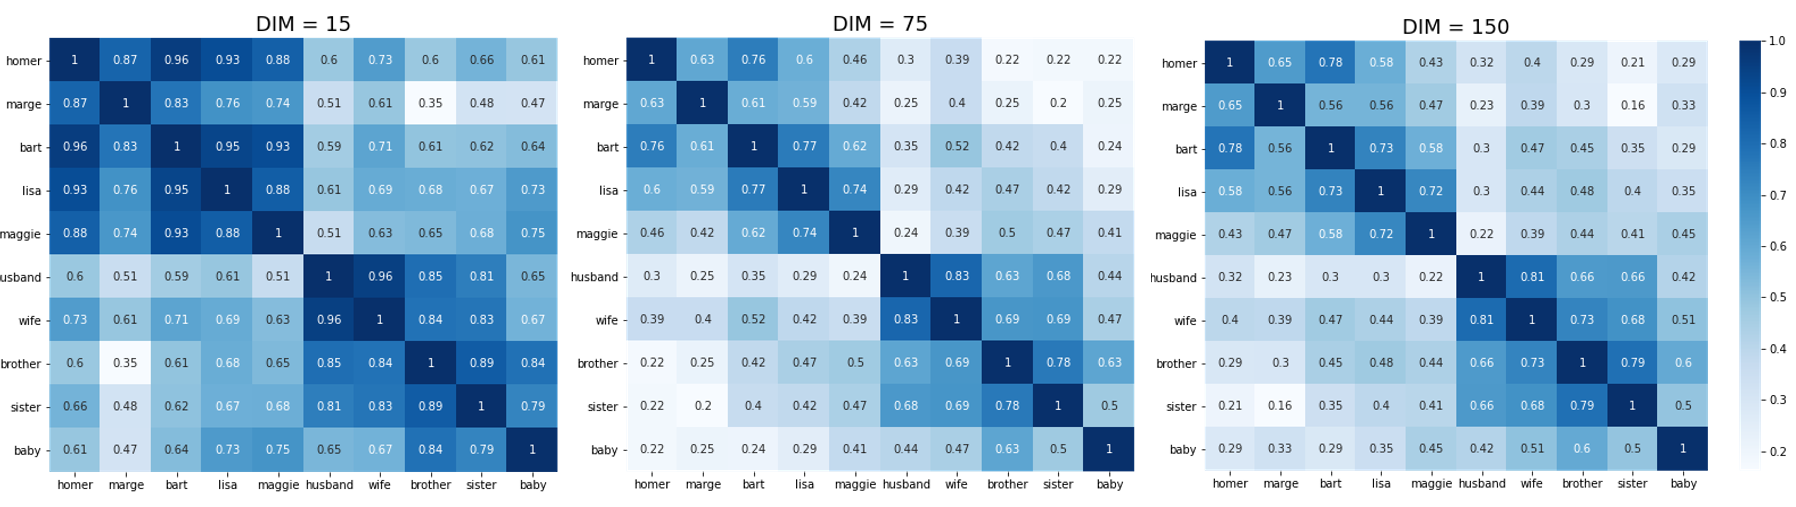
\includegraphics[width=\textwidth]{doc/images/simpsons_sim_matrix.png}
    \caption{Caption}
    \label{fig:simpsons_sim_matrix}
\end{figure}

\subsubsection{Friends Dataset}

\begin{figure}[H]
    \centering
    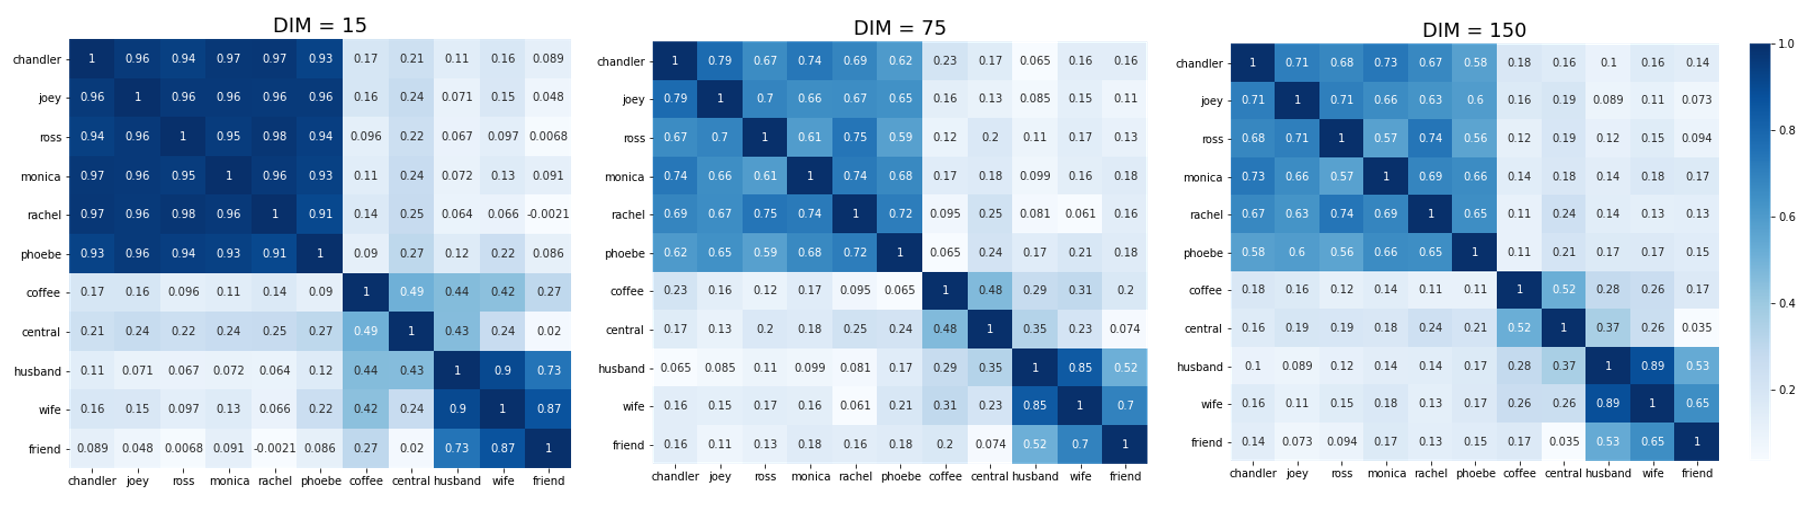
\includegraphics[width=\textwidth]{doc/images/friends_sim_matrix.png}
    \caption{Caption}
    \label{fig:friends_sim_matrix}
\end{figure}
\section{Classification Models (Word2Vec Embeddings)}

\subsection{Simpsons Dataset}

\subsection{Friends Dataset}
\newpage
\section{Classification Models (Trainable Vectorization and Emebddings)}
La clasificación de los modelos en conjunto con su vectorización y los \textit{embeddings} inicia con la búsqueda de los mejores hiper parámetros mediante una búsqueda de grilla modificada. En un principio, la búsqueda de grilla debería variar una serie de hiper parámetros con el fin de encontrar los que producen un mejor modelo. Sin embargo, variar todos los parámetros dentro de una misma búsqueda implica entrenar y evaluar múltiples modelos, lo cual requiere una gran cantidad de tiempo y recursos computacionales. Con el fin de disminuir el tiempo dedicado a la búsqueda de los hiper parámetros se realiza una búsqueda de cada valor de forma independiente. Esta aproximación se ve favorecida por el conocimiento previo del problema y de algunos valores obtenidos en etapas previas del desarrollo del problema.

La búsqueda de los hiper parámetros se hace variando los valores correspondientes a la dimensionalidad del embedding, la longitud de las sentencias y el tamaño del vocabulario. El orden en el cual se realiza esta búsqueda está determinado por el hecho de que se conocen datos de la longitud de las sentencias y del tamaño del vocabulario. En este sentido, el primer parámetro a buscar corresponde a la dimensionalidad del embedding, seguido de la longitud de las sentencias y finalizando con el tamaño del vocabulario. Vale la pena mencionar que otras condiciones relacionadas a los modelos, como lo son instancias de regularización y variaciones en la vectorización, van a ser evaluadas posteriormente.

Para realizar la búsqueda de los parámetros se utiliza un modelo, descrito en la tabla \ref{tab:deep_em_hyper_params}, de una red neuronal completamente conectada (FCN, \textit{Fully Connected Network}). La primera capa de la red corresponde a la de vectorización de texto que oficia como entrada al modelo, recibiendo las sentencias a clasificar. La salida de la capa de vectorización corresponde a una secuencia con una cantidad dada de tokens denotados por \textit{seq\_len}. Una vez se ha vectorizado el texto, este entra a la capa de embedding cuya dimensionalidad va a estar dada por \textit{seq\_len} y \textit{embedding\_dim} que representa la dimensionalidad del embedding. La capa de embedding presenta una salida de dos dimensiones que debe ser ajustada para alimentar las capas densas de la red neuronal. Para dicho ajuste se usa una capa que calcula el promedio global de cada embedding, convirtiendo así la salida de dos dimensiones en un vector con \textit{embedding\_dim} dimensiones. La capa densa de la red contienen un número de neuronas que se calcula con el promedio entre \textit{embedding\_dim} y \textit{output\_dim}, que corresponde al número de clases que serán clasificadas. Finalmente, la última capa contiene \textit{output\_dim} neuronas con el fin de realizar la clasificación correspondiente.

\begin{table}[h]
    \centering
    \begin{tabular}{|l|l|}
        \hline
        \textbf{Tipo de Capa} & \textbf{Características} \\ \hline
        Vectorización de Texto & Denotada por \textit{seq\_len} \\ \hline
        Embedding & Denotada por \textit{seq\_len} y \textit{embedding\_dim} \\ \hline
        Promedio Global de 1D & Convierte los valores a una dimensión \\ \hline
        Densa & Neuronas: promedio entre \textit{embedding\_dim} y \textit{output\_dim} \\ \hline
        Densa & Neuronas: dado por \textit{output\_dim} \\ \hline
    \end{tabular}
    \caption{Definición del modelo para la evaluación y selección de hiper parámetros.}
    \label{tab:deep_em_hyper_params}
\end{table}

La primera etapa de la búsqueda de hiper parámetros se dedicó a fijar la dimensionalidad del embedding. Las posibles dimensiones consideradas fueron de 5, 10, 15, 20, 25, 50, 100 y 150. Las figuras \ref{fig:em_embedding_simpsons} y \ref{fig:em_embedding_friends} presentan respectivamente los resultados para los dos conjuntos de datos: el de \textit{Los Simpsons} y \textit{Friends}. Se puede identificar que los mejores resultados se obtienen con una dimensión de 150 para los dos conjuntos de datos. Vale la pena notar que los modelos para el conjunto de datos de \textit{Friends} demuestran aprendizaje, pero con bajos niveles de recall. 

\begin{figure}
    \centering
    \begin{subfigure}[b]{0.45\textwidth}
        \centering
        
\includegraphics[width=\textwidth]{doc/images/Logo.png}
        \caption{Métricas de evaluación para diferentes dimensiones del embedding en el conjunto de datos de \textit{Los Simpsons}.}
        \label{fig:em_embedding_simpsons}
    \end{subfigure}
    \hfill
    \begin{subfigure}[b]{0.45\textwidth}
        \centering
        
\includegraphics[width=\textwidth]{doc/images/Logo.png}
        \caption{Métricas de evaluación para diferentes dimensiones del embedding en el conjunto de datos de \textit{Friends}.}
        \label{fig:em_embedding_friends}
    \end{subfigure}
    \caption{Métricas de evaluación para la búsqueda de la mejor dimensión del embedding.}
    \label{fig:em_embedding}
\end{figure}

Una vez se ha definido la mejor dimensión para el embedding, se procede a evaluar distintas longitudes de las secuencias. 


\subsection{Simpsons Dataset}

\subsection{Friends Dataset}
\section{Resultados}

\subsection{Simpson dataset}

\subsubsection{Modelos con embedding personalizado}

Los modelos descritos previamente en la sección \ref{sec:deepModels} se implementan como clasificadores para identificar cuál de los personajes principales de Los Simpson dijo un diálogo específico. En este caso se identifican como personajes principales Bart, Homer, Lisa y Marge, siendo las clases 0, 1, 2, 3 respectivamente. Se almacenan los resultados y se muestran los siguientes resultados promediando según modelo, tamaño del embedding y longitud de la secuencia de entrada a la red.\\

\begin{figure}[H]
    \centering
    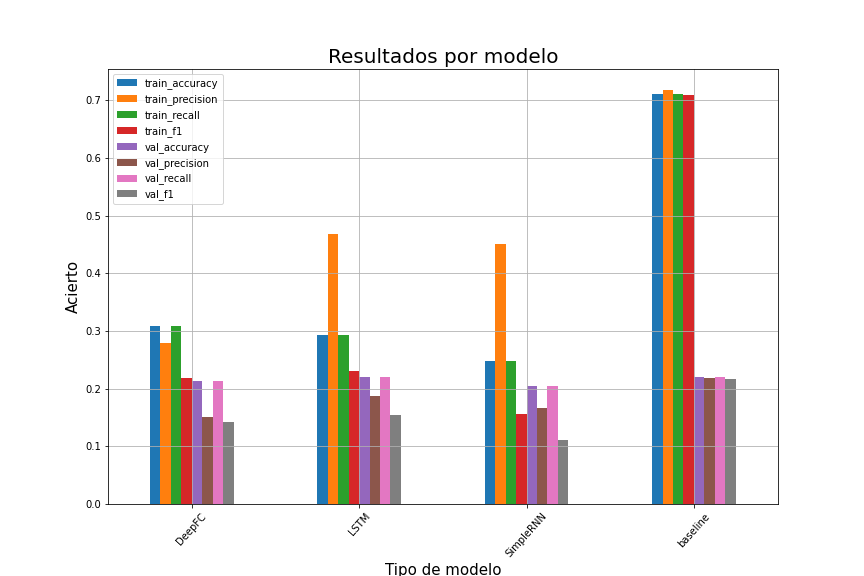
\includegraphics[width=0.9\textwidth]{results/friends/deepModels/sim_res_deep_model.png}
    \caption{Resultados por tipo de modelo}
    \label{fig:sim_deep_model}
\end{figure}

Según la figura \ref{fig:sim_deep_model}, es evidente que el modelo de tipo \textit{baseline} incurre rápidamente en \textit{overfitting}, pues su acierto en los datos de entrenamiento es muy bueno, pero en los de validación es pésimo. En cuanto a los otros modelos su rendimiento es relativamente parejo, destacando una muy buena precisión por parte de los modelos recurrentes  (LSTM y Simple RNN).\\

\begin{figure}[H]
    \centering
    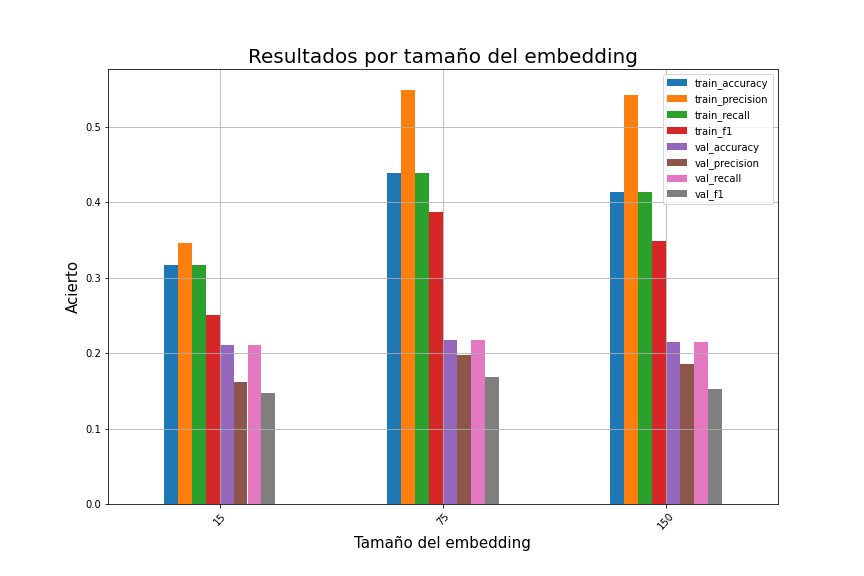
\includegraphics[width=0.9\textwidth]{results/friends/deepModels/sim_res_deep_em_size.png}
    \caption{Resultados por tamaño del embedding}
    \label{fig:sim_deep_em_size}
\end{figure}

Ahora bien, se desea comparar el efecto de los diferentes tamaños de embedding implementados, los cuales corresponden a 15, 75 y 150. Nuevamente, resulta evidente (\textit{véase fig. \ref{fig:sim_deep_em_size}}) que el embedding de tamaño 150 tiende a sobre ajustarse más a los datos de entrenamiento. No obstante, alcanza a dar un resultado ligeramente mejor que los de 15 y 75.\\

\begin{figure}[H]
    \centering
    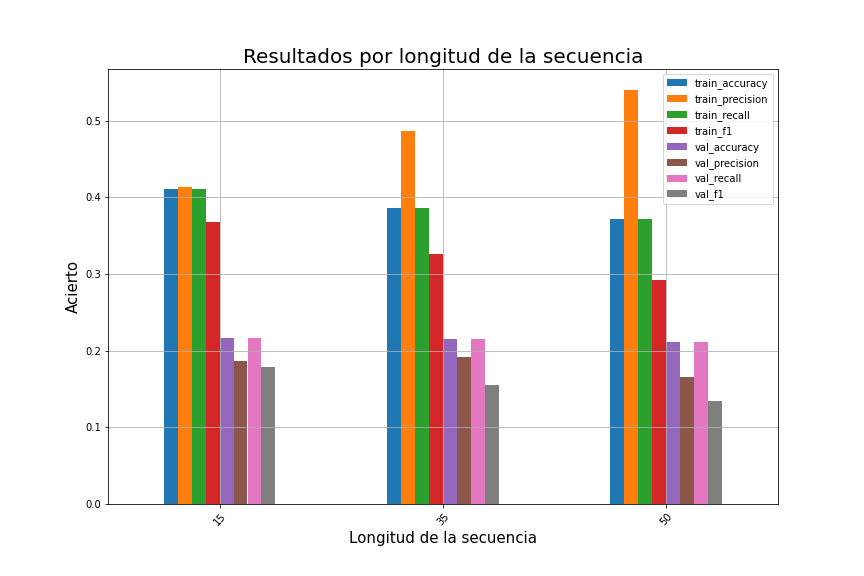
\includegraphics[width=0.9\textwidth]{results/friends/deepModels/sim_res_deep_seq_len.png}
    \caption{Resultados por el tamaño de la secuencia}
    \label{fig:sim_deep_seq_len}
\end{figure}

Finalmente, se desea comparar el efecto de utilizar secuencias de diferente tamaño (15, 35, 50). Los resultados en general son bastante similares favoreciendo un poco el f1 score de secuencias de tamaño 15.\\

Para análisis posteriores, se extrae el mejor modelo con base en el f1 score. Con este modelo se obtienen predicciones sobre datos de validación y de entrenamiento y se reentrena utilizando estos dos grupos de datos para predecir finalmente sobre los datos de test. Con base en todos estas predicciones se obtienen los siguientes resultados:

\begin{itemize}
    \item \textbf{Entrenamiento:}
    \input{results/simpson/deepModels/Train.txt}
    
    \begin{figure}[H]
        \centering
        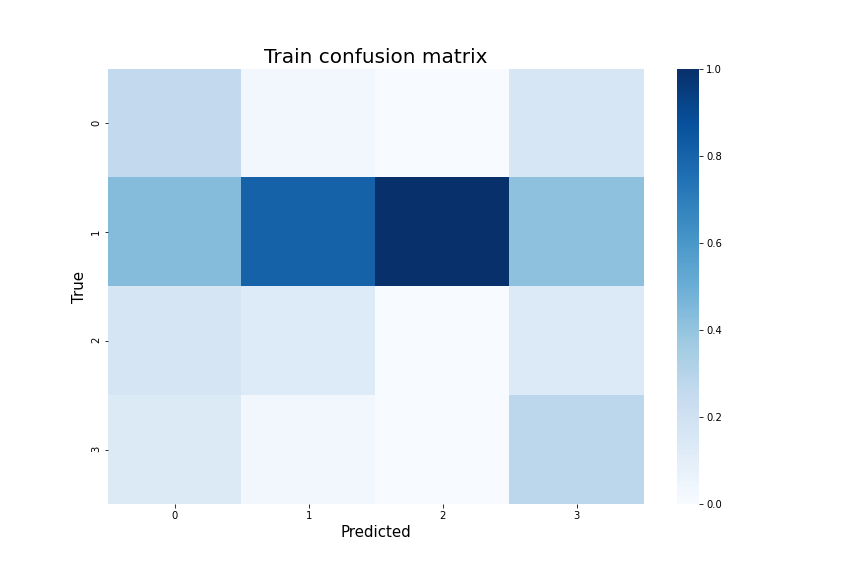
\includegraphics[width=0.9\textwidth]{results/simpson/deepModels/Train.png}
        \caption{Matriz de confusión para entrenamiento en Los Simpson}
        \label{fig:my_label}
    \end{figure}
    
    En el caso de la clase 1 correspondiente a Homer, se puede ver un recall muy bajo, lo que indica la baja certeza al clasificar un modelo como de su clase. Las métricas de las otras clases son ligeramente mejores, especialmente Bart y Marge, edn donde se aprecia un F1 score bastante bueno. En cuanto a la matriz de confusión, se puede ver que en algunos casos la diagonal está más cargada, no obstante, puede ser mejor.
    
    \item \textbf{Validación:}
    \input{results/simpson/deepModels/Validation.txt}
    
    \begin{figure}[H]
        \centering
        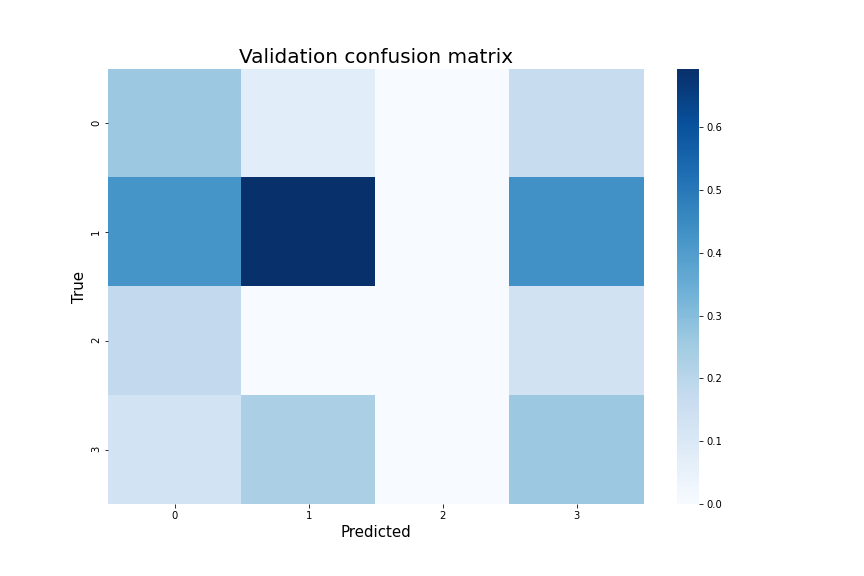
\includegraphics[width=0.9\textwidth]{results/simpson/deepModels/Validation.png}
        \caption{Matriz de confusión para validación en Los Simpson}
        \label{fig:my_label}
    \end{figure}
    
    Se puede apreciar un buen recall tanto para Bart como para Marge al igual que en entrenamiento. Los resultados en general son muy similares a los obtenidos en la etapa previa, como era de esperarse. 
    
    \item \textbf{Test:}
    \input{results/simpson/deepModels/Test.txt}
    
    \begin{figure}[H]
        \centering
        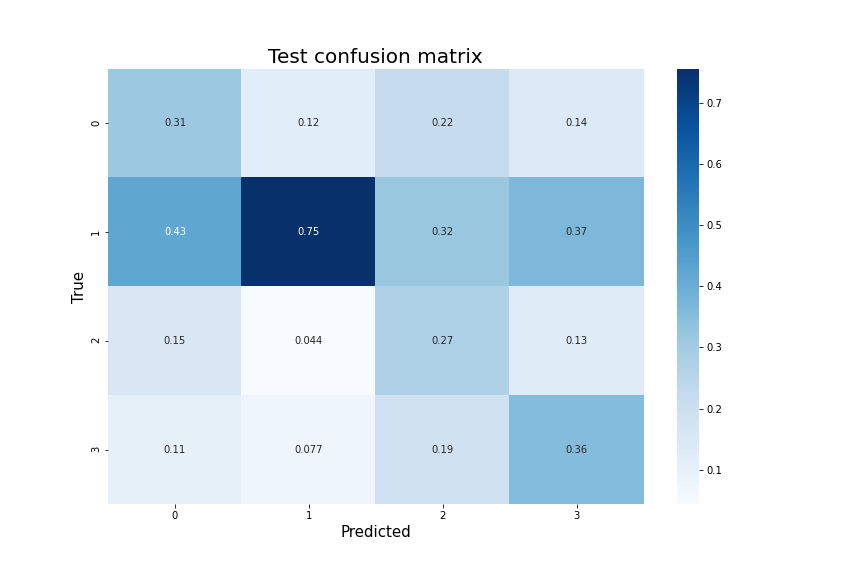
\includegraphics[width=0.9\textwidth]{results/simpson/deepModels/Test.png}
        \caption{Matriz de confusión para test en Los Simpson}
        \label{fig:my_label}
    \end{figure}
    
    En este caso se puede ver una importante y notable mejora en las clases que venían presentando problemas (Homer y Lisa). Se puede apreciar también una mejora en la distribución de la clasificación de la matriz de confusión aunque aún con puntos débiles especialmente en la clase 0 y 3, las cuales antes tenían mejores resultados
    
\end{itemize}

\subsubsection{Modelos con embedding dentro de la red}
La tabla \ref{tab:em_simpsons_global} presenta los resultados de los tipos de modelos considerados para el problema de clasificación del conjunto de datos de \textit{Los Simpsons}. Los resultados de la tabla \ref{tab:em_simpsons_global} provienen de la evaluación del conjunto de prueba sobre el mejor modelo de cada uno de los tipos que fueron puestos a prueba. En términos generales se puede decir que los modelos logran captar suficiente información como para realizar una clasificación dado que su \textit{accuracy} es mayor del 25\% esperado en un clasificador completamente aleatorio. Por otra parte, se tienen los valores de \textit{precision} y \textit{recall} que se combinan en la puntuación F1. Para la \textit{precision} se puede notar que supera el 60\% para todos los tipos de modelos, lo cual indica que estos tienden a presentar un menor número de falsos positivos. Sin embargo, el \textit{recall}, que en ningún caso supera el 40\%, indica que los modelos tienden a presentar falsos negativos.

\begin{table}[H]
    \centering
    \csvreader[%
    tabular={|c|c|c|c|c|},
    table head=\hline \textbf{Modelo} & \textbf{Accuracy} & \textbf{Precision} & \textbf{Recall} & \textbf{F1} \\ \hline,
    late after line=\\ \hline,
    respect underscore = true
    ]%
    {data/results/simpsons_models.csv}%
    {model=\model, accuracy=\acc, precision=\prec, recall=\rec, F1=\fone}
    {\model & \acc & \prec & \rec & \fone}
    \caption{Métricas de evaluación sobre datos de prueba de \textit{Los Simpsons} para los mejores modelos de cada tipo.}
    \label{tab:em_simpsons_global}
\end{table}


\begin{table}[H]
    \centering
    \csvreader[%
    tabular={|c|c|c|c|},
    table head=\hline \textbf{Clase} & \textbf{Precision} & \textbf{Recall} & \textbf{F1} \\ \hline,
    late after line=\\ \hline,
    respect underscore = true
    ]%
    {data/results/simpsons_train.csv}%
    {class=\class, precision=\prec, recall=\rec, F1=\fone}
    {\class & \prec & \rec & \fone}
    \caption{Métricas de evaluación sobre datos de entrenamiento de \textit{Los Simpsons} discriminadas por clase.}
    \label{tab:em_simpsons_train}
\end{table}


\begin{table}[H]
    \centering
    \csvreader[%
    tabular={|c|c|c|c|},
    table head=\hline \textbf{Clase} & \textbf{Precision} & \textbf{Recall} & \textbf{F1} \\ \hline,
    late after line=\\ \hline,
    respect underscore = true
    ]%
    {data/results/simpsons_val.csv}%
    {class=\class, precision=\prec, recall=\rec, F1=\fone}
    {\class & \prec & \rec & \fone}
    \caption{Métricas de evaluación sobre datos de validación de \textit{Los Simpsons} discriminadas por clase.}
    \label{tab:em_simpsons_train}
\end{table}


\begin{table}[H]
    \centering
    \csvreader[%
    tabular={|c|c|c|c|},
    table head=\hline \textbf{Clase} & \textbf{Precision} & \textbf{Recall} & \textbf{F1} \\ \hline,
    late after line=\\ \hline,
    respect underscore = true
    ]%
    {data/results/simpsons_test.csv}%
    {class=\class, precision=\prec, recall=\rec, F1=\fone}
    {\class & \prec & \rec & \fone}
    \caption{Métricas de evaluación sobre datos de prueba de \textit{Los Simpsons} discriminadas por clase.}
    \label{tab:em_simpsons_train}
\end{table}


\subsubsection{Conclusiones}

\subsection{Friends dataset}

Para el caso de Friends, los modelos a implementar son exactamente los mismos. En este caso, cabe resaltar que al ser mayor cantidad de clases, se espera un resultado con desempeño más bajo. Los personajes principales en este caso son Mónica, Joey, Chandler, Phoebe, Ross y Rachel, 0, 1, 2, 3, 4, 5 respectivamente. A continuación, se muestra en consolidado de los resultados.\\

\subsubsection{Modelos con embedding personalizado}

Se puede evidenciar en la figura \ref{fig:fri_deep_model} que nuevamente el modelo \textit{baseline} incurre en \textit{overfitting} rápidamente. En este caso, cabe resaltar que los resultados de SimpleRNN no son tan parejos como los de LSTM, en especial en validación. De igual manera, DeepFC incurre en overfitting, pues sus resultados en entrenamiento mejoran, pero los de validación no se mueven.\\

\begin{figure}[H]
    \centering
    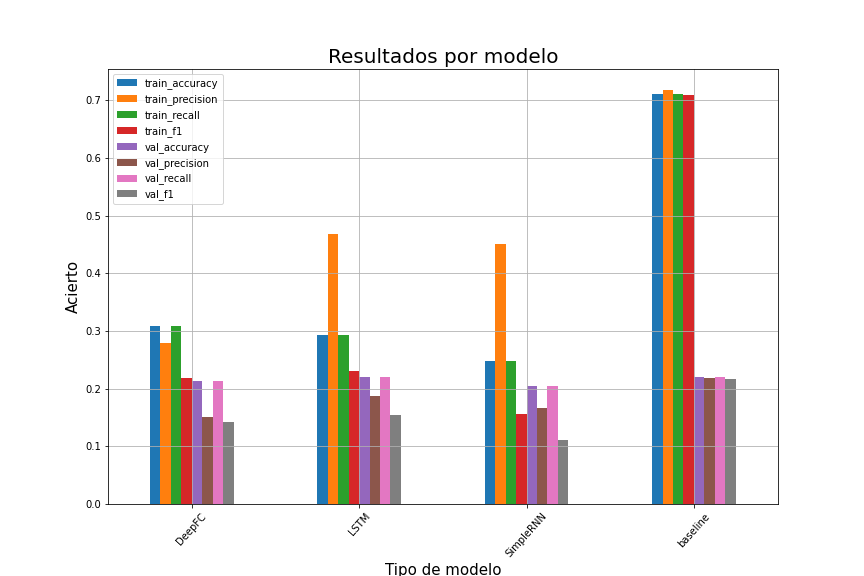
\includegraphics[width=0.9\textwidth]{results/friends/deepModels/sim_res_deep_model.png}
    \caption{Resultados por modelo}
    \label{fig:fri_deep_model}
\end{figure}

En el caso del tamaño del embedding implementado, los resultados son muy similares a los obtenidos para Los Simpson, en tanto a que a medida que se incrementa el embedding hay más posibilidad de sobre ajustar el modelo a los datos de entrenamiento.\\

\begin{figure}[H]
    \centering
    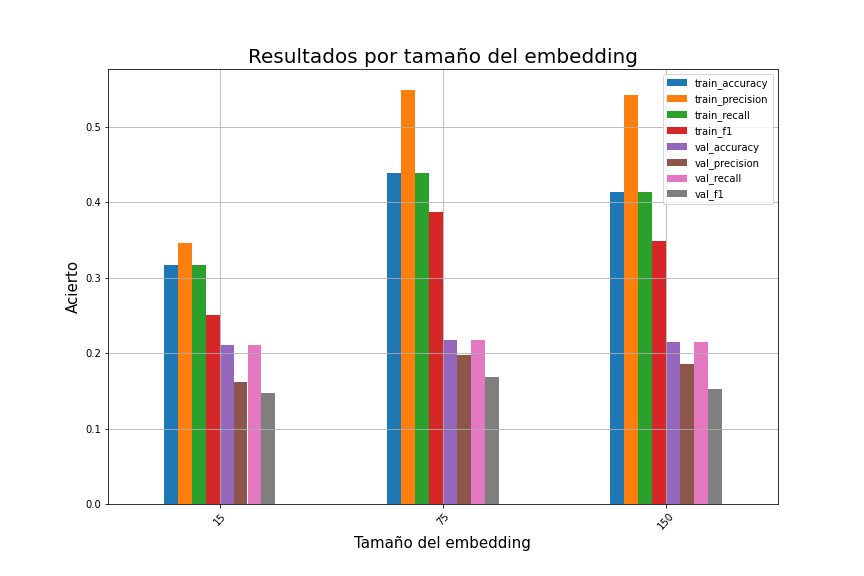
\includegraphics[width=0.9\textwidth]{results/friends/deepModels/sim_res_deep_em_size.png}
    \caption{Resultados por tamaño del embedding}
    \label{fig:fri_deep_em_size}
\end{figure}

Finalmente, en cuanto al tamaño de la secuencia, se observan resultados semejantes en validación con una pequeña diferencia en entrenamiento favoreciendo una secuencia de 15.\\

\begin{figure}[H]
    \centering
    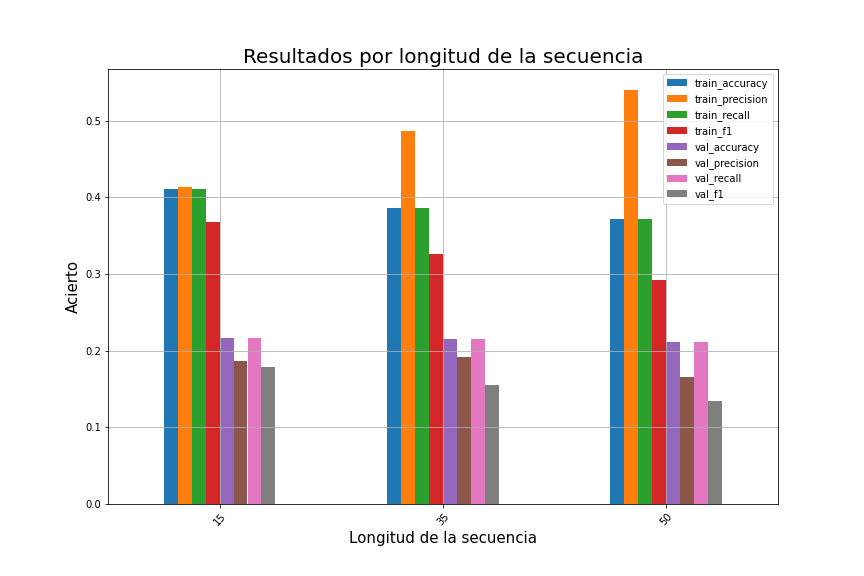
\includegraphics[width=0.9\textwidth]{results/friends/deepModels/sim_res_deep_seq_len.png}
    \caption{Resultados por tamaño de la secuencia}
    \label{fig:fri_deep_seq_len}
\end{figure}

Para análisis posteriores, se extrae el mejor modelo con base en el f1 score. Con este modelo se obtienen predicciones sobre datos de validación y de entrenamiento y se reentrena utilizando estos dos grupos de datos para predecir finalmente sobre los datos de test. Con base en todos estas predicciones se obtienen los siguientes resultados:

\begin{itemize}
    \item \textbf{Entrenamiento:}
    \input{results/friends/deepModels/Train.txt}

    \begin{figure}[H]
        \centering
        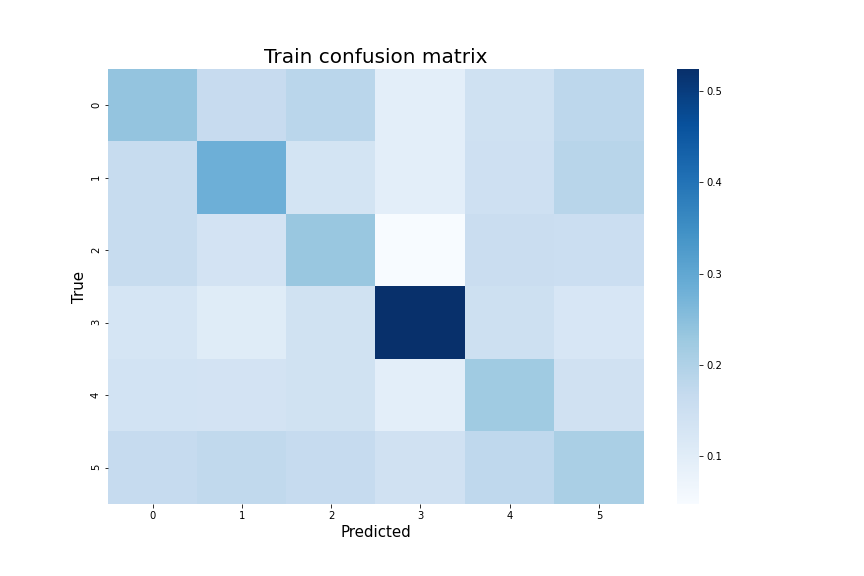
\includegraphics[width = 0.9\textwidth]{results/friends/deepModels/Train.png}
        \caption{Matriz de confusión para entrenamiento de friends}
        \label{fig:my_label}
    \end{figure}
    
    Es claro entonces que hay unas clases cuya precisión es muy alta mientras que su recall es bajo (Joey, Mónica) y por el contrario una clase cuyo recall es alto y su precisión es baja (Chandler). Esto quiere decir que el modelo casi identifica bastantes guiones de Chandler, pero podría decirse que lo asigna como por defecto, pues pocos de los que clasifica como suyos son realmente de su clase. En los restantes personajes sucede que el recall es bajo, mostrando que recupera pocos guiones de los que en realidad son de cada clase. En la matriz de confusión puede verse que la diagonal no resalta, pues hay muchos números de magnitud similar, indicando que el desempeño del modelo es muy aleatorio.

    \item \textbf{Validación:}
    \input{results/friends/deepModels/Validation.txt}

    \begin{figure}[H]
        \centering
        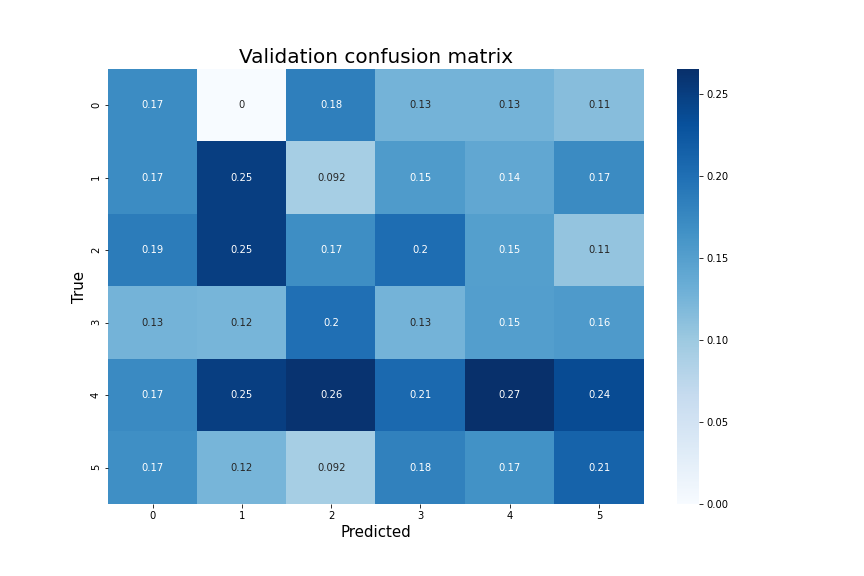
\includegraphics[width = 0.9\textwidth]{results/friends/deepModels/Validation.png}
        \caption{Matriz de confusión para validación de friends}
        \label{fig:my_label}
    \end{figure}
    
    Ahora bien, los resultados descritos previamente se repiten para el caso de validación como era de esperarse. Mostrando que las funciones que describen los datos de entrenamiento y validación son similares, dando lugar a una baja varianza. La matriz de confusión resulta muy mala en especial para la clase 4 donde clasifica sus diálogos como de otros con casi igual probabilidad.
    
    \item \textbf{Test:}
    \input{results/friends/deepModels/Test.txt}

    \begin{figure}[H]
        \centering
        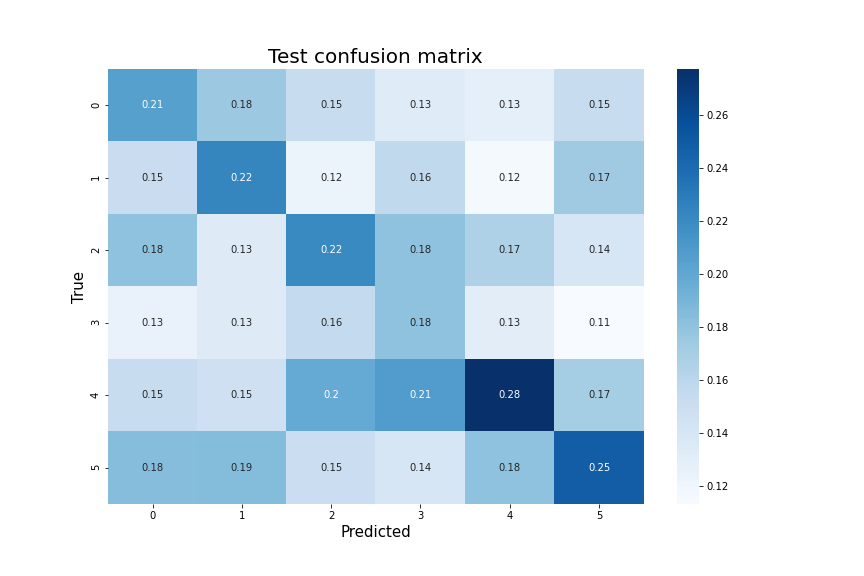
\includegraphics[width = 0.9\textwidth]{results/friends/deepModels/Test.png}
        \caption{Matriz de confusión para Test de friends}
        \label{fig:my_label}
    \end{figure}
    
    Para este caso es pertinente resaltar que, como se describió previamente, se utilizan los datos de entrenamiento y validación para entrenar nuevamente el modelo y se evalúa sobre los datos de test. Es evidente que el resultado de la clasificación es mejor que en las etapas previas, pues la diagonal de la matriz está más cargada.

\end{itemize}



\subsubsection{Modelos con embedding dentro de la red}
La tabla \ref{tab:em_friends_global} presenta los resultados de los tipos de modelos considerados para el problema de clasificación del conjunto de datos de \textit{Friends}. Los resultados de la tabla \ref{tab:em_friends_global} provienen de la evaluación del conjunto de prueba sobre el mejor modelo de cada uno de los tipos que fueron puestos a prueba. En términos generales se puede decir que los modelos logran captar suficiente información como para realizar una clasificación dado que su \textit{accuracy} es mayor del 16.33\% esperado en un clasificador completamente aleatorio. Por otra parte, se tienen los valores de \textit{precision} y \textit{recall} que se combinan en la puntuación F1. Para la \textit{precision} se puede notar que supera el 40\% para todos los tipos de modelos, lo cual indica que estos tienden a presentar un mayor número de falsos positivos. Sin embargo, el \textit{recall}, que en ningún caso supera el 10\%, indica que los modelos tienden fuertemente a presentar falsos negativos.

\begin{table}[H]
    \centering
    \csvreader[%
    tabular={|c|c|c|c|c|},
    table head=\hline \textbf{Modelo} & \textbf{Accuracy} & \textbf{Precision} & \textbf{Recall} & \textbf{F1} \\ \hline,
    late after line=\\ \hline,
    respect underscore = true
    ]%
    {data/results/friends_models.csv}%
    {model=\model, accuracy=\acc, precision=\prec, recall=\rec, F1=\fone}
    {\model & \acc & \prec & \rec & \fone}
    \caption{Métricas de evaluación sobre datos de prueba de \textit{Los Simpsons} para los mejores modelos de cada tipo.}
    \label{tab:em_friends_global}
\end{table}



\subsubsection{Conclusiones}

\newpage
\bibliographystyle{unsrt}
\bibliography{biblist.bib}

\end{document}